\documentclass[11pt,english]{article}
\usepackage{listings}
\usepackage{amsmath}
\usepackage{graphicx}
\graphicspath{ {../} }

\author{Sean Curran \\
\and Stephen Durofchalk \\
\and Zachary Feldman \\
\and Ryan Wails}

\title{EE454 Project 1 Report}
\lstset{language=Matlab}
\renewcommand{\thesection}{\alph{section}}

\begin{document}
\maketitle

\newpage
\section{Project Summary}

\section{Procedural Approach}

\section{Experimental Observations}

\section{Performance Evaluation}

\section{Further Exploration}
\subsection{Test Cases}
To test the robustness/accuracy of the training outside of the given data set, additional test images were gathered and fed into the RNN.  Images were rescaled to thumbnail size (32x32x3) with the Matlab command
\begin{lstlisting}
thumbnail = imresize(img, [32 32]);
\end{lstlisting}

\noindent
110 images total were collected; 100 fell into the preexisting image classes, 10 contained scenes not falling into any preexisting class.  Running these new 10 images through the RNN yielded the following results:\\

\begin{tabular}{ | c | c | c |}
  \hline
  Image \# & Image Contents & RNN Classification \\
  \hline		
  Image 1 & Tree in Field & Horse (8) \\
  Image 2 & Winter Mountain Scene & Ship (9) \\
  Image 3 & Ryan and Zach & Bird (3) \\
  Image 4 & Steve & Frog (7) \\
  Image 5 & Sean & Cat (4) \\
  Image 6 & Desktop Computer & Automobile (2) \\
  Image 7 & Football on Field & Deer(5) \\
  Image 8 & Robert Collins & Truck (10) \\
  Image 9 & Old Main & Bird(3) \\
  Image 10 & Penn State Logo & Truck (10)\\
  \hline  
\end{tabular}

\subsection{Reclassification}
An attempt was made to distinguish these 10 images from the rest of the data set (i.e. reclassify these 10 images as unknown).  Let $V$ be the vector of output probabilities from the RNN for each image.  Let $C$ be the classification of the image producing probability vector $V$.  Originally, we have\\~\\
\begin{math}
p_i \in V \\
p_{max} = \max(p_1, p_2,...,p_{10}) \\
C = i $ given $ p_i = p_{max}
\end{math}

~\newline\noindent
To reclassify the images we use\\
\noindent
\begin{math}
p_{max} = \max(p_1,p_2,...,p_{10}) \\
P = \{p_1,p_2,...,p_{10}\} \setminus \{p_{max}\} \\
p_{2max} = \max(P) \\~\\
\begin{cases}
C = i $ given $ p_i = p_{max} & $for	$ p_{max} - p_{2max} > 0.25 \\
C = 11 & $otherwise$
\end{cases}
\end{math}
~\\~\\
Less precisely, the difference between the two peak responses was thresholded by .25; so, if there were two strong responses, the image is reclassified as unknown.

\subsection{Results After Reclassification}
In the confusion matrix below, classes 1 through 10 are the same classifications.  Class 11 identifies an unknown image class. \\\\
\begin{tabular}{ | c | c | c | c | c | c | c | c | c | c | c | c | c | }
\hline
	 & CNN
Class & 1 & 2 & 3 & 4 & 5 & 6 & 7 & 8 & 9 & 10 & 11 \\ \hline
	True 
Class &  &  &  &  &  &  &  &  &  &  &  &  \\ \hline
	1 &  & 3 & 0 & 0 & 0 & 0 & 0 & 0 & 0 & 1 & 0 & 6 \\ \hline
	2 &  & 1 & 2 & 0 & 0 & 0 & 0 & 0 & 0 & 2 & 0 & 5 \\ \hline
	3 &  & 1 & 0 & 2 & 0 & 0 & 0 & 0 & 0 & 0 & 0 & 7 \\ \hline
	4 &  & 0 & 0 & 0 & 1 & 0 & 0 & 0 & 0 & 0 & 0 & 9 \\ \hline
	5 &  & 0 & 0 & 0 & 0 & 0 & 0 & 0 & 1 & 0 & 0 & 9 \\ \hline
	6 &  & 0 & 0 & 2 & 0 & 0 & 0 & 0 & 0 & 0 & 0 & 8 \\ \hline
	7 &  & 0 & 0 & 0 & 1 & 0 & 0 & 1 & 0 & 0 & 0 & 8 \\ \hline
	8 &  & 0 & 0 & 1 & 1 & 0 & 0 & 1 & 4 & 0 & 0 & 3 \\ \hline
	9 &  & 0 & 0 & 0 & 0 & 0 & 0 & 0 & 0 & 5 & 0 & 5 \\ \hline
	10 &  & 0 & 0 & 0 & 0 & 0 & 0 & 0 & 0 & 0 & 5 & 5 \\ \hline
	11 &  & 0 & 0 & 0 & 0 & 0 & 0 & 0 & 0 & 1 & 0 & 9 \\ \hline
\end{tabular}

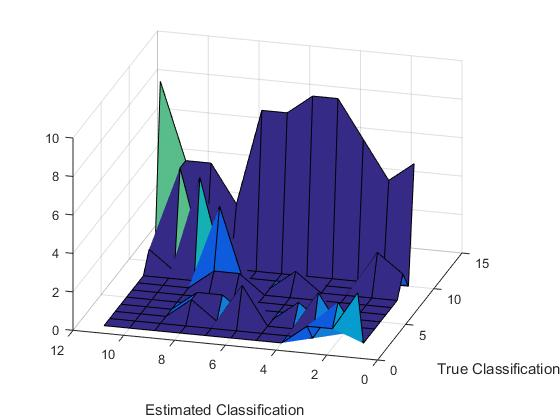
\includegraphics[scale=0.6]{confexp}
~\\~\\
\textbf{Accuracy = 29.09\%}
\\
The reclassification metric does well in replacing the 10 new images in the unknown category, but also places images that were previously correctly classified in the unknown category.  Other metrics tested were
\begin{enumerate}
\item Thresholding on the number of classes that had a response above 0.1 (the mean value for random classification)
\item Taking the spatial derivative of the probability vector; this metric actually produces zero-mean Gaussian noise with a very small standard deviation.
\end{enumerate}

\section{Member Contributions}


\end{document}